\def\baselinestretch{1}

\chapter{Appendix Numerical Linear Algebra}
$M_{m,n}(\field{F})$ denotes the vector space of matrices over
the field $\field{F}$.

\[A \in M_{n,n}(\dblf) \; b \in \dblf^n,  \exts x  \ni \; Ax=b \,
\;\texttt{iff}\; det(A)=0\]

$\mathbf{X} \in M_{mn}(\field{R})$ is positive definite if $
v^{t} X v > 0 \fall v \in \field{R}^n$.  We can construct
positive definite symmetric matrices by by forming
$\mathbf{X}^{t} \mathbf{X}$ where $\mathbf{X}$ is an orthogonal
(full rank) matrix.

Horner's rule is a method for evaluating a polynomial at a
point in $O(n)$ time. Straightforward evaluation of a n degree
polynomial is done in $O(n^{2})$ time. Simply rewrite the
function $f(x)= \sum\limits_{i=0}^{n-1} {a}_i x^{i}$ as
$f(x)=(\ldots (a_{n-1}x + a_{n-2} )x +  \ldots + a_1)x+a_0$

\section{The min max characterization of eigenvalues}
This is a variational characterization of the eigenvalues of compact operators on a Hilbert space. Let $H \st H=H^\dag$ The Rayleigh quotient is defined by $R(x) =  \frac{<Hx,x>}{\norm{x}^2}$ Let $\sigma(H) ={\lambda_i}$, then $\forall S_k \in \dblr^n$ we have
\begin{equation*}
  \underset{x \in S_k \norm{x}=1}{max} <Hx,x> \geq \lambda_k
\end{equation*}
which implies
\begin{equation*}
\underset{S_k}{inf}  \underset{x \in S_k \norm{x}=1}{max} <Hx,x> \geq \lambda_k
\end{equation*}
Equality above is achieved when $S_k = spn{\mu_k}$ where $\mu_k$ is the kth eigenvector of $H$.

The min max theorem is that
\begin{equation*}
\lambda_1 \leq R(x) \leq \lambda_n
\end{equation*}




\section{The Discrete Fourier Transform on $\ell^2(\dblz_{N_1})$} Let $z \in \dblz_{N_1} ,\!
z=(z(0),z(1),\ldots,z(N_1-1))$.  We index from 0 instead of 1
for convenience of presenting the FFT. Define
\begin{equation*}
\widehat{z(m)}=\sum\limits_{k=0}^{N_1-1} z(k)e^{ \frac{-2 \pi
\imath k m}{N_1}}
\end{equation*}
The map $\hat \!: \ell^2(\dblz_{N_1}) \rightarrow
\ell^2(\dblz_{N_1})$ is the Fourier Transform. The vectors
\begin{equation*}
E_0,E_1, \ldots,E_{N_1 -1}  :\!  E_m(n)=\frac{e^\frac{-2 \pi
\imath m n}{N_1}}{\sqrt{N_1}}
\end{equation*}
form an orthonormal basis for $\ell^2(\dblz_{N_1})$. The
vectors $ \frac{E_0}{N_1},\frac{E_1}{N_1}, \ldots,\frac{E_{N_1
-1}}{N_1}$ form an orthogonal basis called the Fourier Basis.

Extend the indices over $\dblz_{N_1}$ to $\dblz$ by considering
$\dblz_{N_1}$ to be the algebraic group $\dblz mod N_1$.  Then
we can define the translation operator
\begin{equation*}
(R_l z)(n)=z(n-l).
\end{equation*}
We can also define the convolution operator with this extended
notion of $\dblz_{N_1}$;
\begin{equation*}
z * w = \sum \limits_{k=0}^{N_1-1} z(m-n)W(n)
\end{equation*}
The Fourier Multiplier Operator $T_{(m)}$ where $m \in
\ell_2{\dblz_{N_1}}$ is given by
\begin{equation*}
T_{(m)}=(m\hat z)\check{}
\end{equation*}

Fourier Inversion Formula:
\begin{equation*}
z(m)=\frac {1}{N_1}\sum\limits_{k=0}^{N_1-1} \hat{z(k)} e^{
\frac{2 \pi \imath k m}{N_1}}
\end{equation*}

Parsevall's Relation:
\begin{equation*}
<z,w>=\frac{1}{N_1}<\hat z,\hat w>
\end{equation*}

Plancherel's Formula: Parsevall's relation with $w=z$.

Representation in the Fourier Basis:
\begin{equation*}
z=\sum \limits_{k=0}^{N_1-1} \hat{z(k)} F_k
\end{equation*}

The effect of the translation operator is to rotate the phase
of the Fourier Transform:
\begin{equation*}
(R_l z)\hat(k)=e^{ \frac{2 \pi \imath k l}{N_1}}\widehat{z(k)}
\end{equation*}

The effect of conjugation is to reflect the Fourier Transform:
\begin{equation*}
(\overline{z})\hat(k)=\overline{\hat z(-k)}
\end{equation*}


The Convolution Operator is equivalent to a Fourier Multiplier
Operator:
\begin{equation*}
b * z=(m \hat z )\check{} \! : m=\hat b
\end{equation*}

\section{Multiresolution analysis} Basis functions of a linear
subspace $V_j \subset L^2(\Omega)$ are
defined by a scaling function $\phi$ 

%bbcrevisit - insert the class of admissable scaling fn's for prefect reconstruction, then address frames
via the following procedure;
\begin{gather*}
\phi_{ij}(x) = \phi(2^{-j} x-i)  \\
V_j = span \{ \phi_{ij} \} \\
W_{j+1}= V_j \ V_{j+1}^\bot \\
\hdots V_{j+1} \subset V_j \subset \hdots \subset V_0 \subset \hdots V_{-j}  \subset \hdots \\
V_j=V_{j+1} \oplus W_{j+1} x \in W_{j+1} \Rightarrow \exts
{a_l} \;\; x=\sum_l \{a_l\} \phi_{jl}
\end{gather*}
A basis for $W_{ij}$ is constructed from a mother wavelet
$\psi$.

\section{Voroni Tesselations}
A centroidal Voronoi tessellation is a Voronoi tessellation where the
generating points are the centroids of the corresponding regions.
Applications Voronoi tessellations can be found in image compression,
clustering, quadrature, and finite difference methods. distribution of
resources.  The dual of the Voroni tessellation in $\dblr^2$ is the Delaunay
triangulation.

The example below is a simulated example of resource allocation in $\dblr^2$
A partition of a Random walk in $\dblr^2$ obtained by calculating the Voroni
tessellation and associated Delaunay triangulation on the k-means centroids.

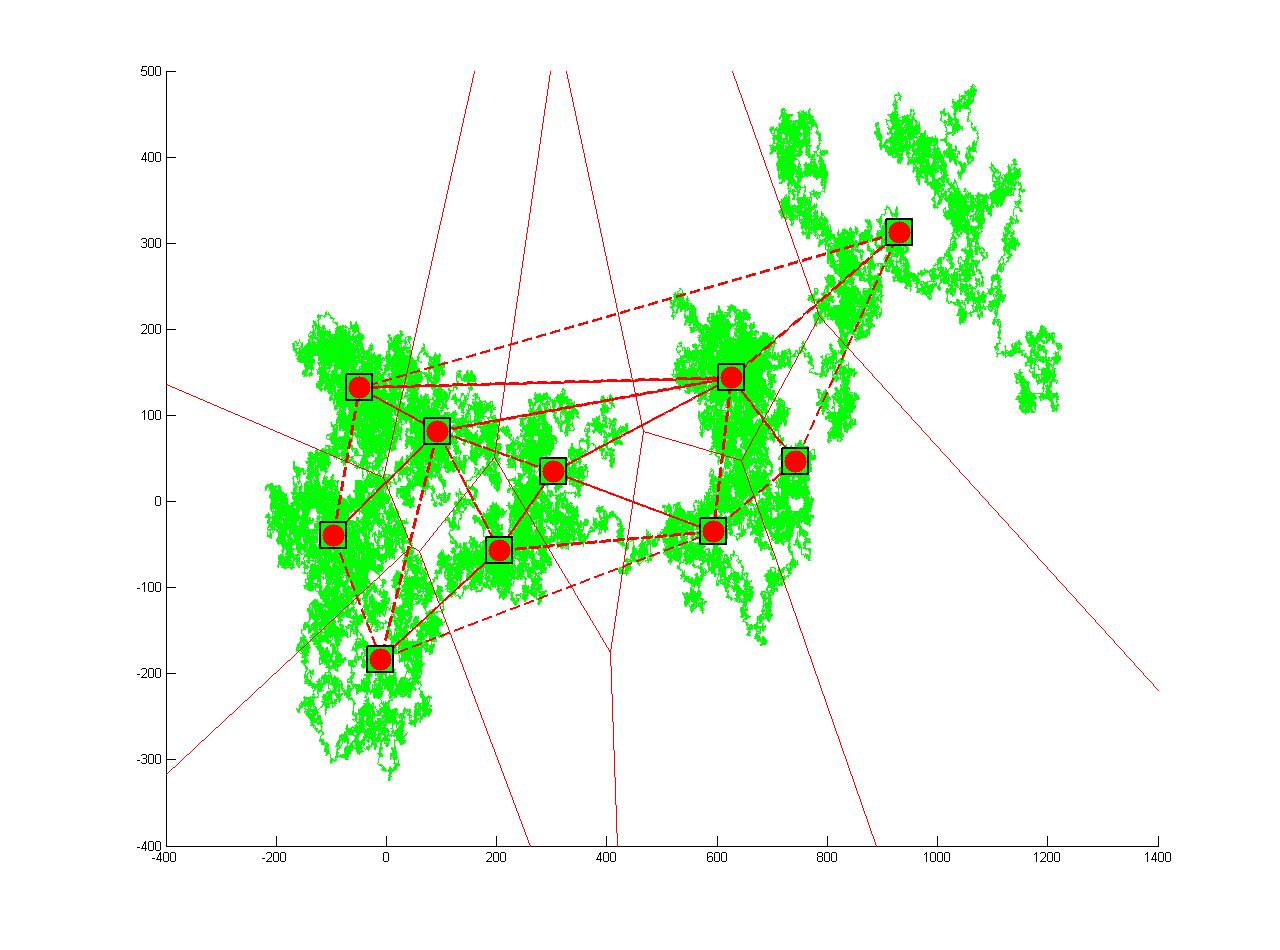
\includegraphics[width=8.0cm,height=8.0cm]{Figures/ClusteringRW/rw_1000000_delauney_kmens_convex_hull_voroni_onKM.jpg}


\section{The Matrix Exponential}
The matrix exponential of a matrix $\mat{A}$ is defined as
\begin{align*}
  e^{\mat{A}}
  &= \mat{I} + \mat{A} + \frac{\mat{A}^2}{2!} + \dots \\
  &= \sum_{k = 0}^\infty \frac{\mat{A}^k}{k!}.
\end{align*}

The Pade approximation to
$e^{\mat{A}}$ is
\begin{displaymath}
  e^{\mat{A}} \approx R(\mat{A}),
\end{displaymath}
with
\begin{align*}
  R_{pq} (\mat{A})
  &= (D_{pq}(\mat{A}))^{-1} N_{pq}(\mat{A}) \\
  \intertext{where}
  D_{pq}(\mat{A})
  &= \sum_{j=1}^p \frac{(p+q-j)! p!}{ (p+q)!j!(p-j)!}\, \mat{A}^j \\
  \intertext{and}
  N_{pq}(\mat{A})
  &= \sum_{j=1}^q \frac{(p+q-j)! q!}{ (p+q)!j!(q-j)!}\, \mat{A}^j.
\end{align*}
See \cite{Moler78nineteendubious} for a detailed accounting of this and other matters regarding the calculation of the matrix exponential.
%\citet{Moler78nineteendubious} \citep*{Moler78nineteendubious} \citep{Moler78nineteendubious} \citet*{Moler78nineteendubious}
